\documentclass[a4paper, 12pt]{article}

\usepackage[brazil]{babel}
\usepackage[utf8]{inputenc}
\usepackage{hyperref} % criar hyperlinks
\usepackage{listings} % utilizado para dar highlight em código
\usepackage[dvipsnames]{xcolor}
\usepackage{graphicx} % importar imagens
\usepackage[export]{adjustbox}
\usepackage[top=3cm, bottom=2cm, left=3cm, right=2cm]{geometry}
\renewcommand{\baselinestretch}{1.5} % espaçamento entre linhas
\setlength{\parskip}{0.5cm} % espaçamento entre paragrafos
\setlength{\parindent}{2cm} % recuo do parágrafo
\usepackage{times}


\lstdefinestyle{customc}{ %custom color para código do arduino
  belowcaptionskip=1\baselineskip,
  backgroundcolor=\color{lightgray},
  breaklines=true,
  frame=single,
  xleftmargin=\parindent,
  language=C,
  showstringspaces=false,
  basicstyle=\footnotesize\ttfamily,
  keywordstyle=\bfseries\color{ForestGreen},
  commentstyle=\itshape\color{darkgray},
  identifierstyle=\color{blue},
  stringstyle=\color{gray},
  breaklines=true,
  morekeywords={bool},
}

\title{Etapas e dificuldades}
\author{Victor Vieira Paulino
\and
Arthur Cicuto Pires}
\date{\today}

\begin{document}

\maketitle

\section{Módulo do Ponto de Ônibus}

\subsection{Hardware}

\begin{enumerate}
\item HM-10 - Bluetooth 4.0 BLE module
\item Arduino Uno
\end{enumerate}

Arduino Uno é utilizado apenas como ponte para configurar o módulo HM-10. A ligação deve seguir o diagrama abaixo.

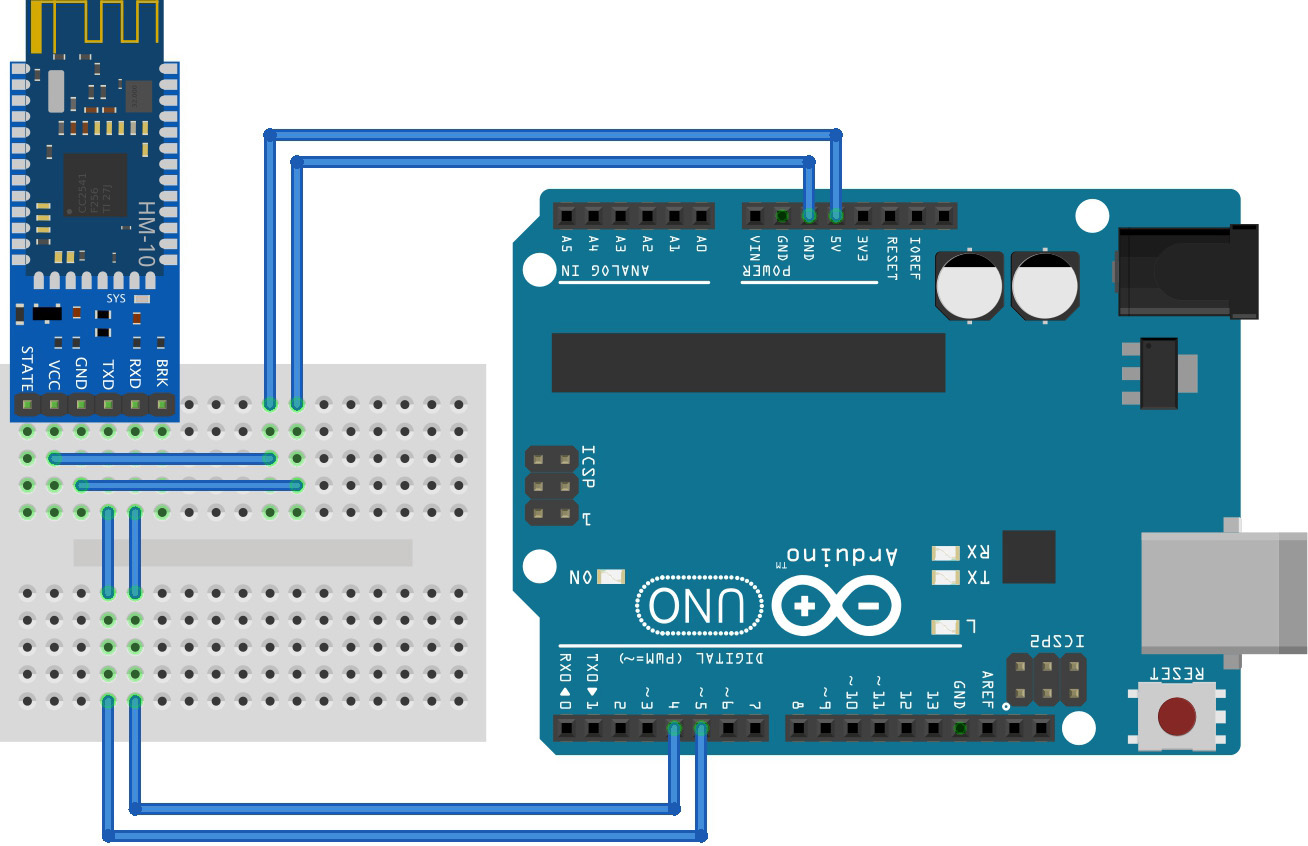
\includegraphics[width=10cm, center]{images/arduino-hm10}

\subsection{Software}

\begin{itemize}
\item Arduino IDE 1.8.3 ou superior. 
\end{itemize}

\subsection{Configuração}

Conecte o arduino Uno ao computador e compile o código abaixo utilizando a IDE do arduino.

\lstinputlisting[style=customc]{codes/arduino-code.ino}

Após compilador, utilizando o Serial Monitor da IDE, execute os comandos AT na seguinte ordem:

Obs: Quanto menor o tempo de envio, maior a economia de energia.

\begin{enumerate}
\item AT+RENEW //Coloca nos padrões de fábrica
\item AT+RESET //Reinicia para aplicar os padrões de fábrica
\item AT+MARJ0xNNNN //Define o valor Marjor
\item AT+MINO0xNNNN //Define o valor Minor
\item AT+NAMEMeuBeacon //Define o nome do Beacon
\item AT+ADVI5 //Define tempo de envio. 5 = 546.25 millisegundos
\item AT+ADTY3 //Define como não pareável
\item AT+IBEA1 //Habilita como Beacon
\item AT+DELO2 //Configura para apenas emitir sinal
\item AT+PWRM0 //Habilita auto-sleep para economizar energia
\item AT+RESET
\end{enumerate}


Após configurado, pode ser ligado em uma bateria 3v para utilização.

\subsection{Referências}

\href{ftp://imall.iteadstudio.com/Modules/IM130614001_Serial_Port_BLE_Module_Master_Slave_HM-10/DS_IM130614001_Serial_Port_BLE_Module_Master_Slave_HM-10.pdf}{HM-10 Bluetooth 4.0 BLE module Datasheet}
\\
\href{https://www.arduino.cc/en/main/software}{Arduino IDE}
\\
\href{https://github.com/metractive/beacon-study}{Repositório da Metractive - Como construir Beacons}

\section{Módulo do Ônibus}

\subsection{Hardware}

\begin{itemize}
\item Intel Edison
\item Raspberry Pi 3
\item Tela LCD 7" (em breve)
\item NEO u-blox 6 GPS Modules
\end{itemize}

\subsubsection{Intel Edison}

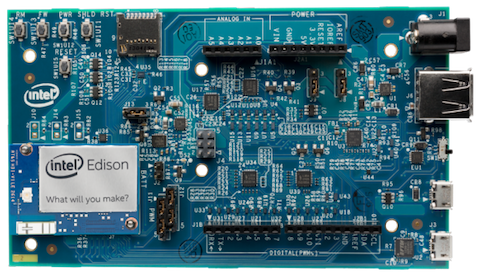
\includegraphics[width=10cm, center]{images/intel-edison-arduino-kit}

Inicialmente foi adotado o Intel Edison com placa de expansão arduino. Foi escolhido devido a fácil acesso a um exemplar e ótimo hardware. Ele conta com WiFi, Bluetooth, portas I/O, processador Intel Atom de 500 MHz, 1GB de memória RAM DDR3 e 4GB eMMC. \\
Sua utilização foi fácil e não obtivemos nenhuma dificuldade em instalar o sistema que escolhemos.


Problemas encontrados em adotar como solução:
\\

\textbf{Preço}

Embora tenha um ótimo hardware e uma empresa séria por trás da sua construção, o preço, em 07/2017, que gira em torno de R\$ 600,00, não justifica sua adoção como a melhor solução para o projeto já que existem alternativas com preços melhores e bom desempenho.
\\

\textbf{Ausência de controlador gráfico}

Uma das features do projeto é emitir alertas visuais para o motorista por meio de telas LCDs. A placa Intel Edison nos permite fazer alertas visuais utilizando LEDs e afins. 
\\

\textbf{Descontinuidade da placa pela Intel}

em 07/2017, a Intel anunciou a descontinuidade do desenvolvimento de algumas placas que fabrica. O Intel Edison foi uma delas.

\subsubsection{Raspberry Pi 3}

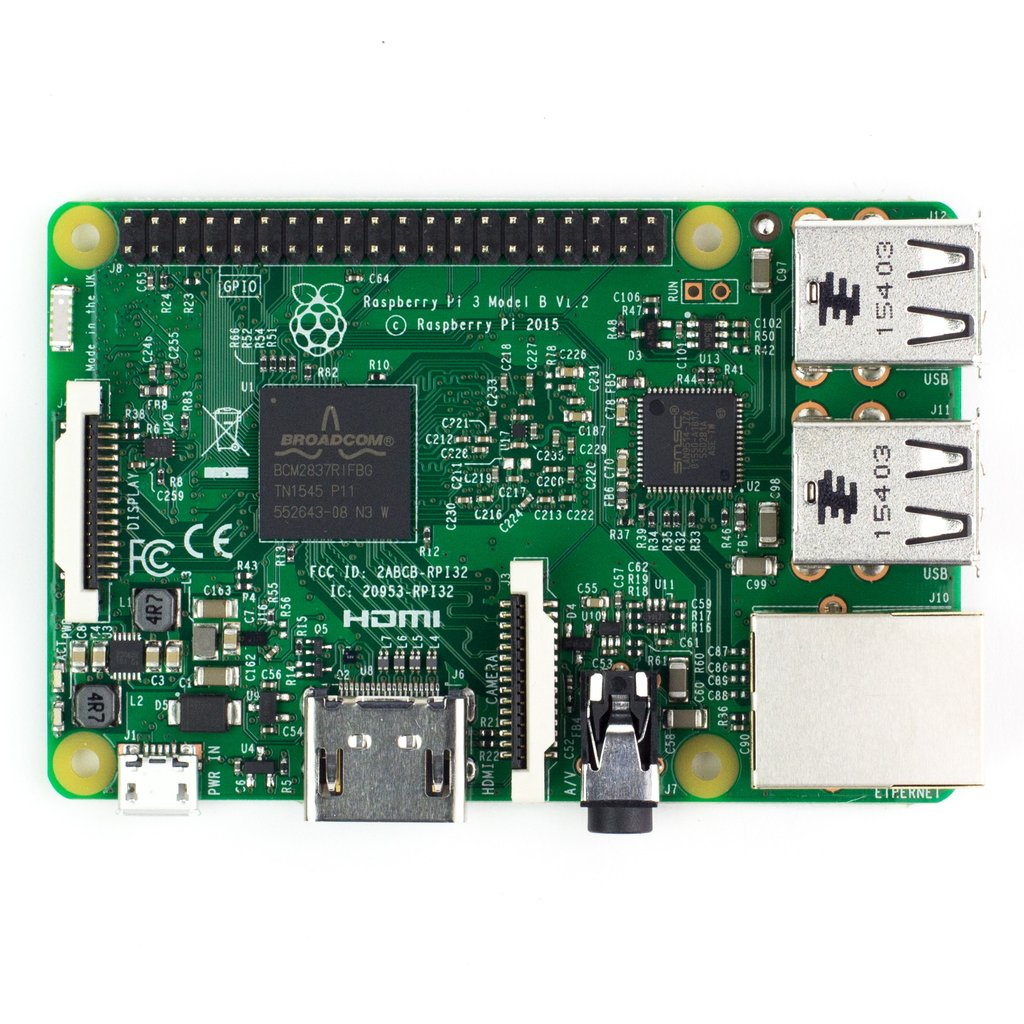
\includegraphics[width=10cm, center]{images/raspberry-pi}

Testes realizados no Raspberry Pi 3 demonstraram ser uma boa alternativa ao Intel Edison. Foi fácil a instalação do sistema e a placa vem com saída HDMI permitindo utilizar telas LCD para fazer os alertas visuais.
Seu preço, em 08/2017, gira em torno de R\$ 150,00, 1/4 do preço do Intel Edison. Seu hardware contém boas especificações:

\begin{itemize}
\item Quad Core 1.2GHz Broadcom BCM2837 64bit CPU
\item 1GB RAM
\item BCM43438 wireless LAN and Bluetooth Low Energy (BLE) on board
\item 40-pin extended GPIO
\item 4 USB 2 ports
\item 4 Pole stereo output and composite video port
\item Full size HDMI
\item CSI camera port for connecting a Raspberry Pi camera
\item DSI display port for connecting a Raspberry Pi touchscreen display
\item Micro SD port for loading your operating system and storing data
\item Upgraded switched Micro USB power source up to 2.5A
\end{itemize}

Embora tenha um hardware com especificações superiores ao Intel Edison, não houve ganho de desempenho ao rodar o sistema, devido a ausência de algoritmos complexos no sistema. Assim, a grande vantagem de se utilizar o Raspberry Pi 3 ao invés do Intel Edison, é seu baixo custo e recurso de chip gráfico.

\subsubsection{Módulo NEO u-blox 6 GPS}

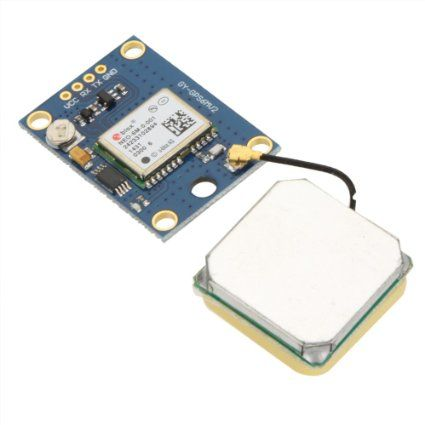
\includegraphics[width=10cm, center]{images/neo-6m}

Para realizar o rastreamento do ônibus foi adotado o módulo NEO u-blox 6 GPS Modules, devido a compatibilidade com as placas que contém o sistema embarcado e preço acessível. 

\textbf{Localização}

Uma característica desse módulo é trabalhar com GPS, fazendo comunicação direta com no mínimo 3 satélites para triangular sua posição com mais precisão. Alguns módulos disponíveis no mercado trabalham com A-GPS, que usam torres de telefonia móvel para conhecer sua posição.
O uso do GPS trás maior precisão, porém demora mais para estabelecer conexão com satélites. O A-GPS fornece a localização com menor tempo, porém com menor precisão e a um custo mais alto.

\textbf{Comunicação}

O módulo realiza comunicação UART (Universal Asynchronous Receiver/Transmitter), o que permite fácil comunicação com as placas utilizadas para testes.

\textbf{Preço}

Seu preço, em 08/2017, gira em torno de R\$ 60,00 e pode ser encontrado com facilidade na internet para venda. 


\subsection{Software}

\subsubsection{Sistema Operacional}

\textbf{Android Things}
Em 2016 o Google anunciou o Android Things, uma versão do Android voltada para IoT (Internet of Things). Ele é, atualmente, uma versão do Android Marshmallow reduzida. Sua escolha foi devido a facilidade de embarcar em placas como o Raspberry Pi e Intel Edison, e a variedade de recursos que já estão disponíveis no SO que facilitam o desenvolvimento do módulo, como o recurso LocationManager. \textbf{[Detalhar mais essa parte]}

\subsubsection{IDE}

Foi escolhido o Android Studio como IDE do projeto. Ela é desenvolvida pela IntelliJ e tida pelo Google como ferramenta oficial de desenvolvimento para aplicativos Android.

\subsubsection{Linguagem}

O Google tem duas linguagens de primeiro nível para desenvolvimento Android: Java e Kotlin. Para esse projeto adotamos a linguagem Kotlin, que possui sintaxe muito simplificado em comparação ao Java. Embora Java tenha sido a primeira linguagem oficial para desenvolvimento, Kotlin oferece acesso aos mesmo recursos do sistema.
Algumas bibliotecas disponíveis, desenvolvidas por terceiros, ainda não migraram para o Kotlin, obrigando a implementar algumas classes em Java. Como Kotlin tem interoperabilidade com Java, não existe nenhum impeditivo de utilizar Kotlin e eventualmente alguma classa Java.

\subsubsection{Arquitetura}

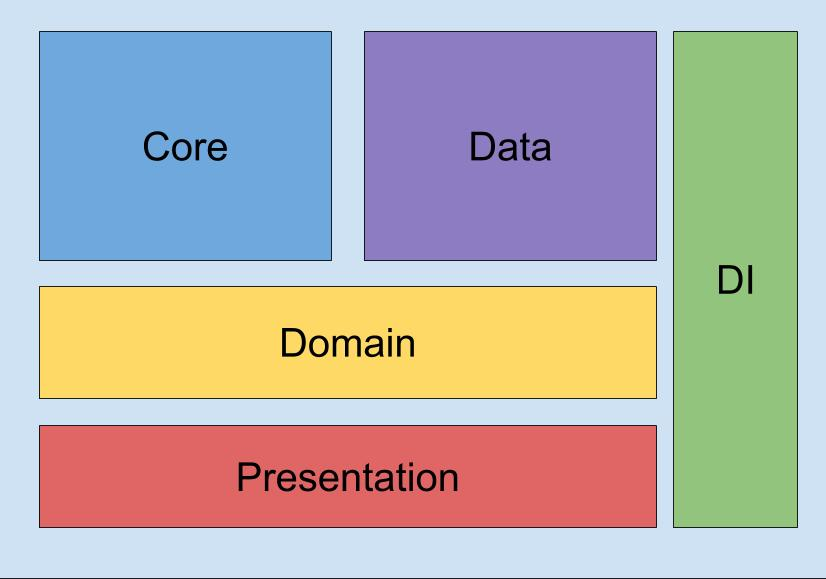
\includegraphics[width=10cm, center]{images/brick_diagram_bus_tracker}

Para desenvolvimento do software, foi adotado o padrão \textit{Clean Archtecture}. É um padrão que visa um maior desacoplamento das classes e distruibui bem as responsabilidades.

\begin{description}

\item[Core] Não contém nenhuma lógica de negócio. Esta camada provê informações comuns, como configurações estáticas da placa a toda a aplicação. Possui também algumas classes e interfaces bases.

\item[Data] Responsável por prover dados para toda aplicação. Ela adota o Padrão de Arquitetura \textit{Repository}, tendo uma interface de acesso aos dados. Uma grande vantagem em utilizar essa camada com esse padrão de arquitetura, é o respeito a responsabilidade única, um dos princípios do \textit{SOLID}. Ela encapsula toda lógica de busca de dados, assim, caso uma classe precise de algum dado específico, ela solicita através da interface de comunicação e a classe que implementa a interface, cuida de toda lógica de busca de dado, seja um dado armazenado localmente, em cache ou em um servidor remoto. Tudo fica transparente para a classe que solicitou o dado.

\item[Domain] Esta camada encapsula toda regra de negócios da aplicação. Toda vez que é necessário realizar processamentos em dados para satisfazer funcionalidades, é feito por esta camada.

\item[Presentation] Responsável por toda interface gráfica. Toda lógica de criação de telas e interceptação de interações do usuário com o aplicativo, é feito aqui. Quando é necessário procurar dados para exibir ao usuário, é feito solicitações deles para a camada Domain ou Data para que seja possa exibir os dados.
 
\end{description}

\subsection{Referências}

%links do intel edison
\href{https://software.intel.com/en-us/iot/hardware/edison}{Site Oficial Intel Edison}\\
\href{http://download.intel.com/support/edison/sb/edisonmodule_hg_331189004.pdf}{Datasheet Intel Edison}\\
\href{https://www.embarcados.com.br/placas-intel-edison-galileo-e-joule-serao-descontinuadas/}{Anúncio do fim da produção do Intel Edison}\\
%links do raspberry pi
\href{https://www.raspberrypi.org/products/raspberry-pi-3-model-b/}{Site Oficial Raspberry Pi}\\
\href{https://www.raspberrypi.org/documentation/hardware/computemodule/RPI-CM-DATASHEET-V1_0.pdf}{Datasheet Raspberry Pi 3}\\
%links do módulo GPS
\href{https://www.u-blox.com/sites/default/files/products/documents/NEO-6_DataSheet_(GPS.G6-HW-09005).pdf}{Datasheet NEO u-blox 6 GPS Modules}\\
%android things
\href{https://developer.android.com/things/index.html}{Site Oficial Android Things}\\
\href{https://developer.android.com/things/hardware/edison.html}{Configuração do Android Things no Intel Edison}\\
\href{https://developer.android.com/things/hardware/raspberrypi.html}{Configuração do Android Things no Raspberry Pi 3}\\

\section{Aplicativo}

\subsubsection{Telas}

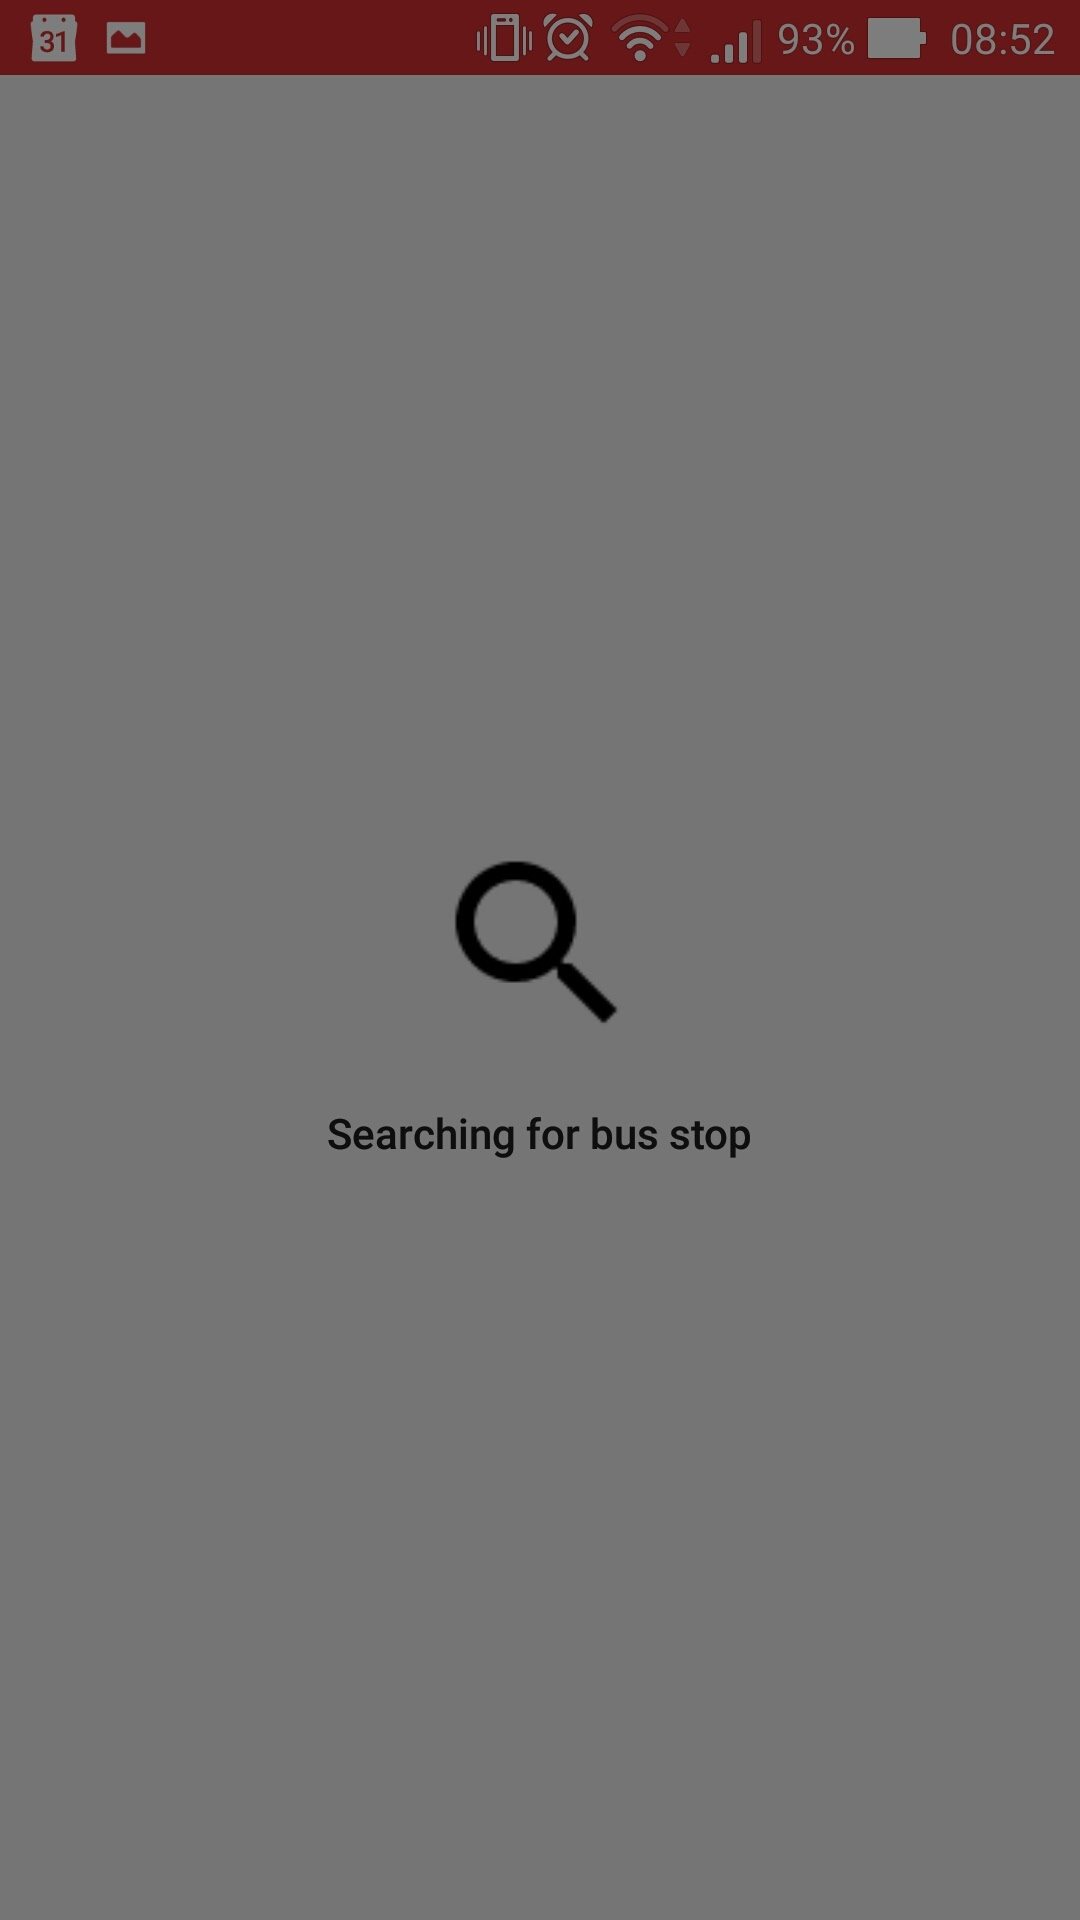
\includegraphics[width=5cm, center]{images/beacon_searching_bus_stop}
\\
\\
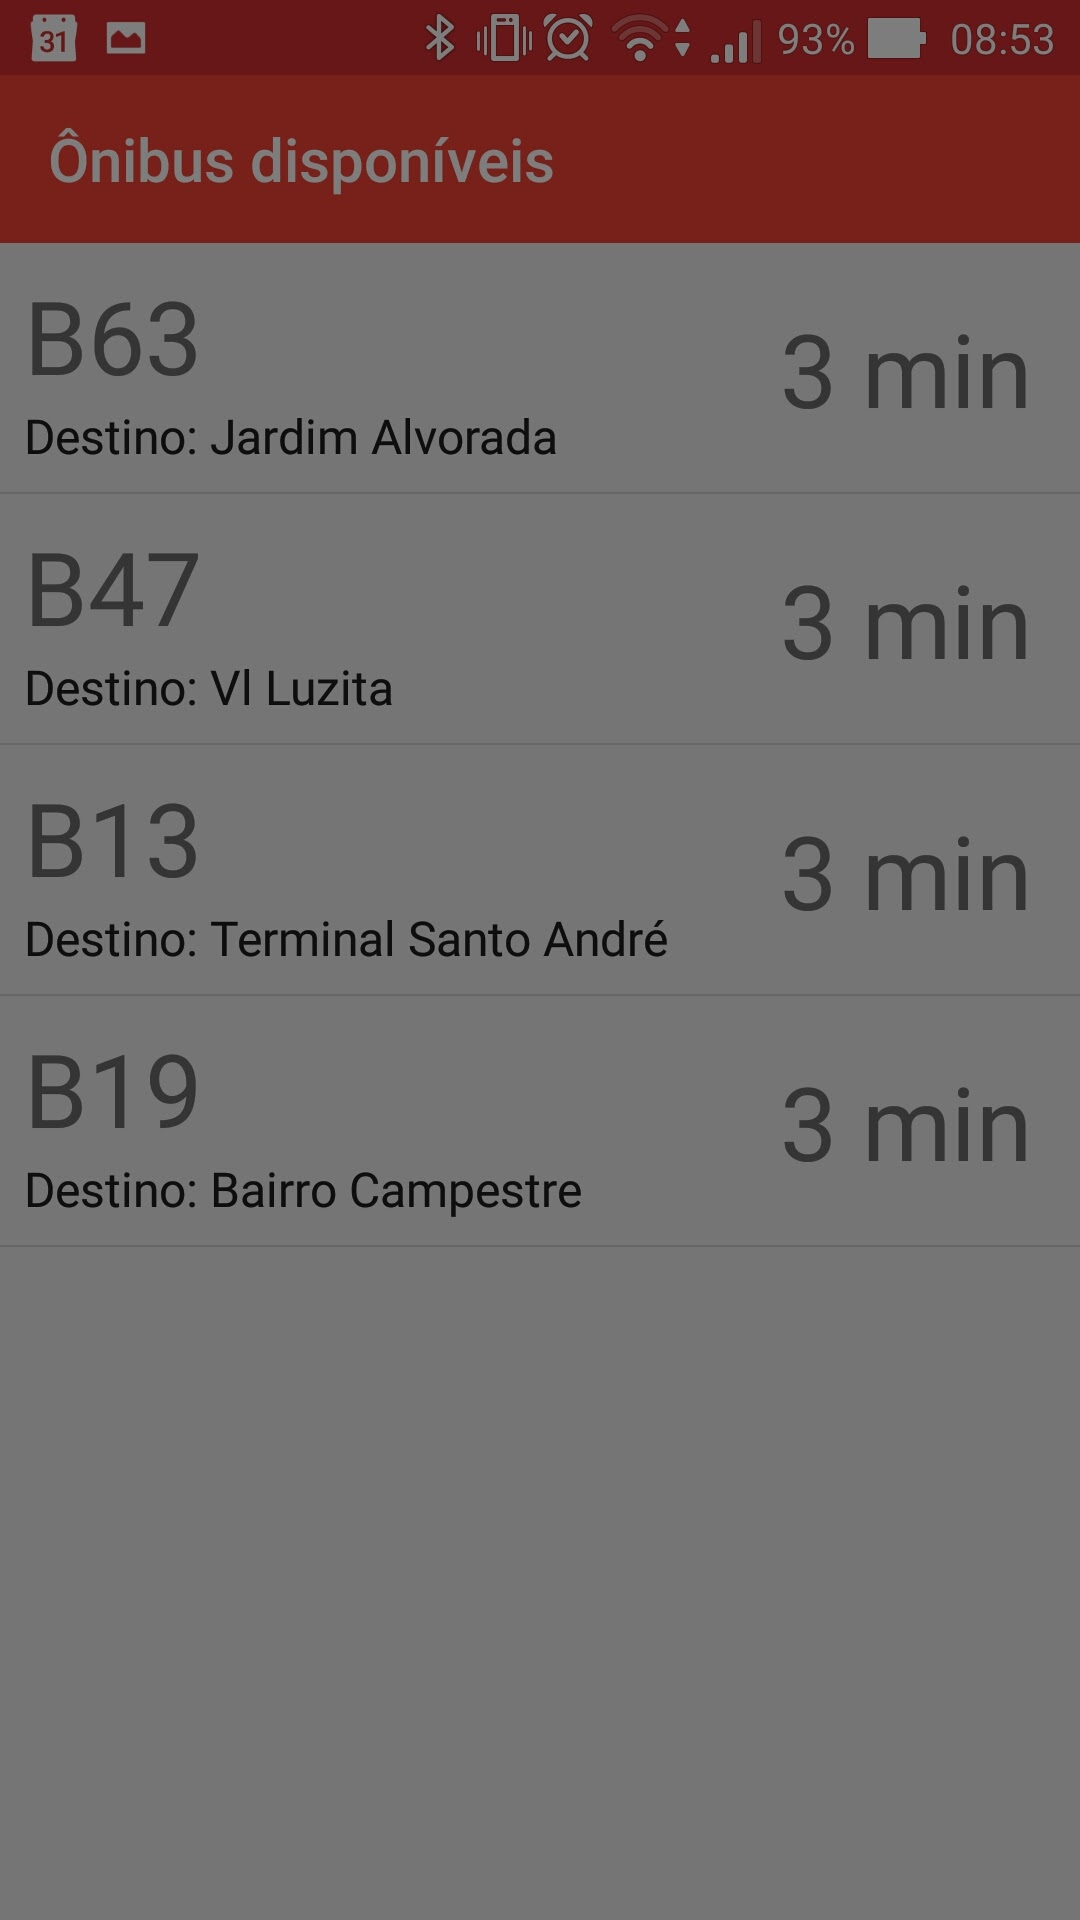
\includegraphics[width=5cm, center]{images/beacon_list_bus}
\\
\\
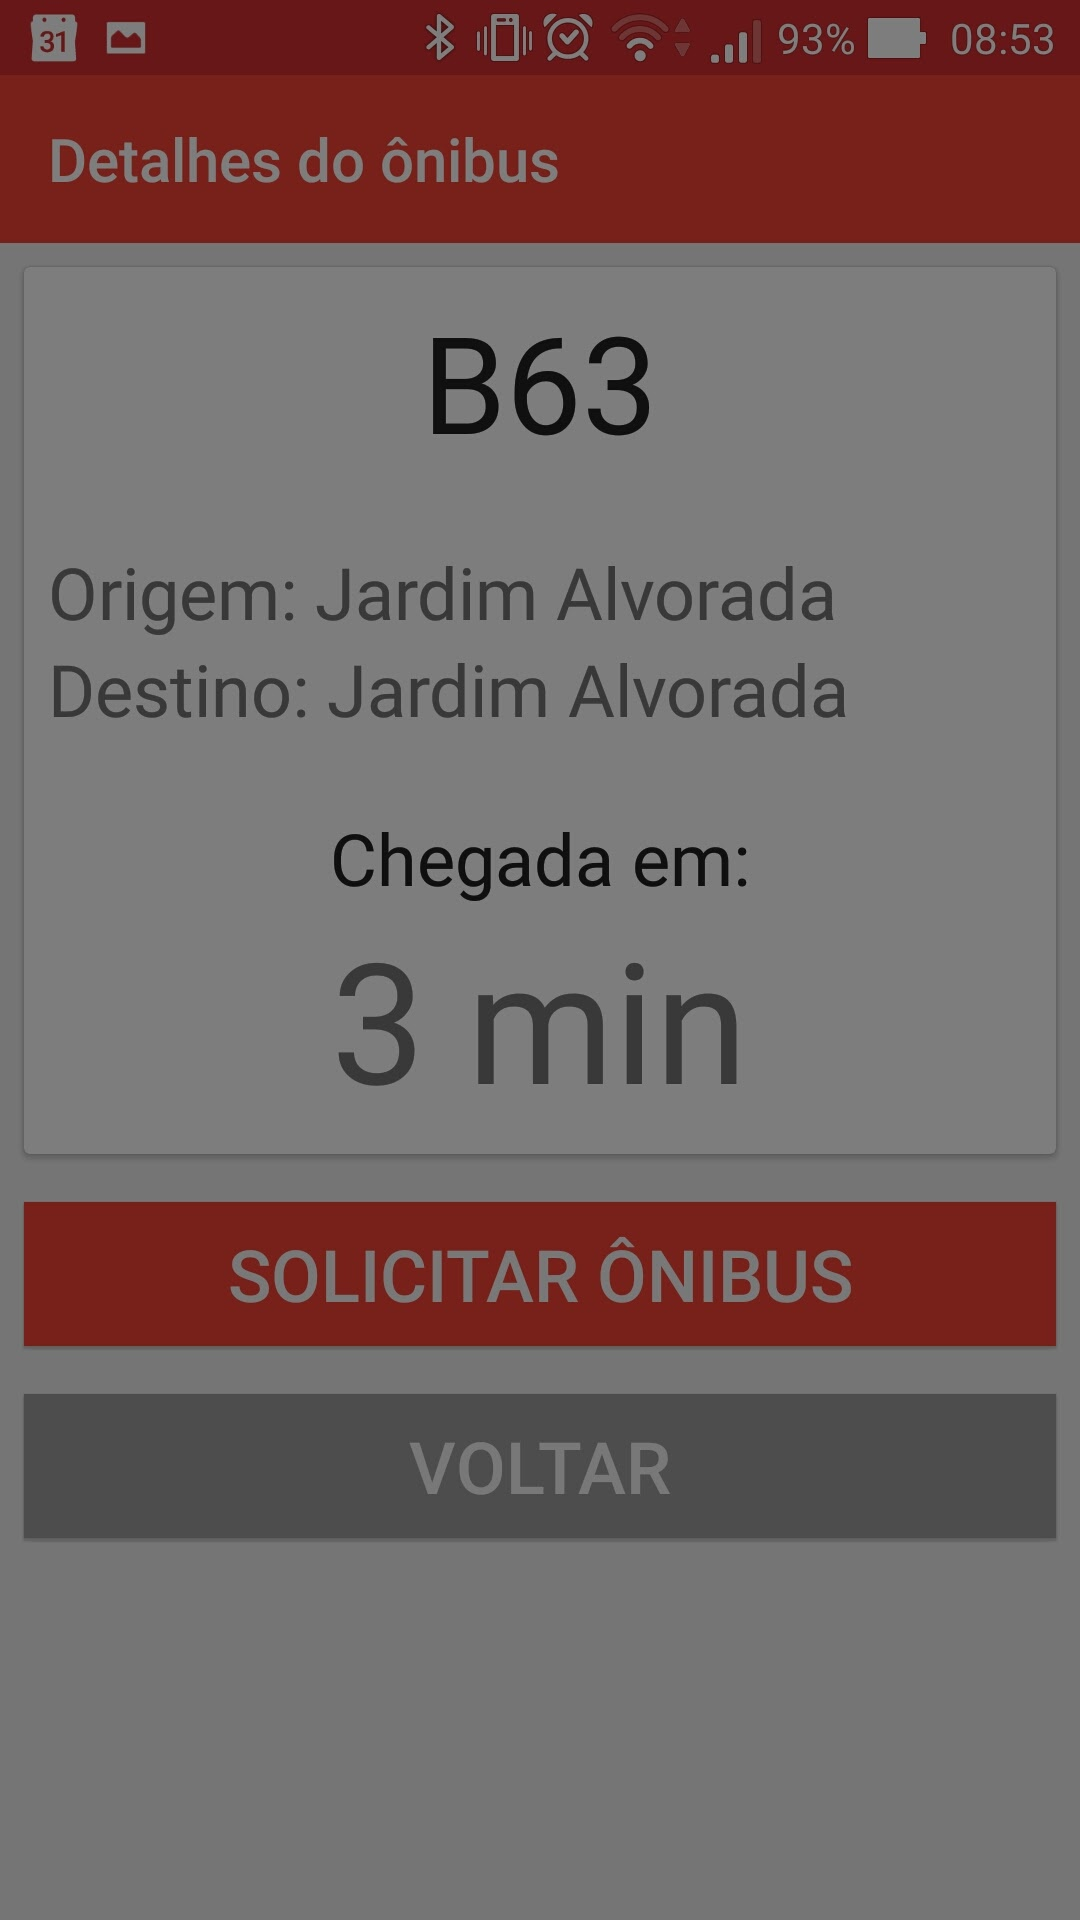
\includegraphics[width=5cm, center]{images/beacon_detail_bus}

\subsubsection{IDE}

Foi escolhido o Android Studio como IDE do projeto. Ela é desenvolvida pela IntelliJ e tida pelo Google como ferramenta oficial de desenvolvimento para aplicativos Android.

\subsubsection{Linguagem}

O Google tem duas linguagens de primeiro nível para desenvolvimento Android: Java e Kotlin. Para esse projeto adotamos a linguagem Kotlin, que possui sintaxe muito simplificado em comparação ao Java. Embora Java tenha sido a primeira linguagem oficial para desenvolvimento, Kotlin oferece acesso aos mesmo recursos do sistema.
Algumas bibliotecas disponíveis, desenvolvidas por terceiros, ainda não migraram para o Kotlin, obrigando a implementar algumas classes em Java. Como Kotlin tem interoperabilidade com Java, não existe nenhum impeditivo de utilizar Kotlin e eventualmente alguma classa Java.

\subsubsection{Arquitetura}

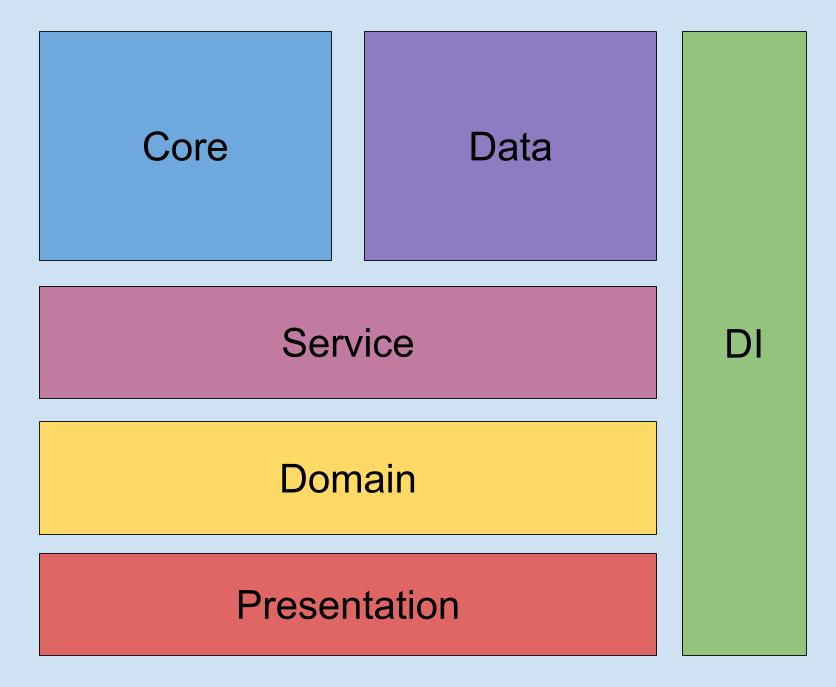
\includegraphics[width=10cm, center]{images/brick_diagram_beacon}

Para desenvolvimento do software, foi adotado o padrão \textit{Clean Archtecture}. É um padrão que visa um maior desacoplamento das classes e distruibui bem as responsabilidades.

\begin{description}

\item[Core] Não contém nenhuma lógica de negócio. Esta camada provê informações comuns, como configurações estáticas da placa a toda a aplicação. Possui também algumas classes e interfaces bases.

\item[Data] Responsável por prover dados para toda aplicação. Ela adota o Padrão de Arquitetura \textit{Repository}, tendo uma interface de acesso aos dados. Uma grande vantagem em utilizar essa camada com esse padrão de arquitetura, é o respeito a responsabilidade única, um dos princípios do \textit{SOLID}. Ela encapsula toda lógica de busca de dados, assim, caso uma classe precise de algum dado específico, ela solicita através da interface de comunicação e a classe que implementa a interface, cuida de toda lógica de busca de dado, seja um dado armazenado localmente, em cache ou em um servidor remoto. Tudo fica transparente para a classe que solicitou o dado.

\item[Domain] Esta camada encapsula toda regra de negócios da aplicação. Toda vez que é necessário realizar processamentos em dados para satisfazer funcionalidades, é feito por esta camada.

\item[Presentation] Responsável por toda interface gráfica. Toda lógica de criação de telas e interceptação de interações do usuário com o aplicativo, é feito aqui. Quando é necessário procurar dados para exibir ao usuário, é feito solicitações deles para a camada Domain ou Data para que seja possa exibir os dados.
 
\end{description}

\section{\itshape Web service}

\subsection{Linguagem}

Para o desenvolvimento do \textit{web service} foi escolhida a utilização da pilha MEAN, que engloba quatro tecnologias para desenvolvimento \textit{web} que possuem como base a linguagem JavaScript.


\subsubsection{JavaScript}

JavaScript é uma linguagem de programação \textit{client-side}, utilizada para manipular os comportamentos de uma página, controlando o HTML e o CSS. Outra característica dela, é que ela é uma linguagem orientada à eventos.
Para explicar melhor o que são eventos, é importante citar que uma página HTML utiliza tags para representar seus elementos, podendo conter menus, botões e formulários em seu corpo. Cada elemento possui alguns atributos, sendo alguns desses atributos de eventos, como por exemplo o \textit{onClick} que realiza alguma função caso o elemento referente seja clicado pelo usuário.
Tais funções podem ser desenvolvidas em JavaScript, entrando aqui para dizer qual comportamento a página terá ao disparo do evento.\\

\subsection{\itshape MEAN stack}

A pilha \textit{MEAN} é um conjunto de \textit{frameworks} desenvolvidos em JavaScript, que englobam os lados do cliente, do servidor e do banco de dados. Por possuírem a mesma linguagem como base, os elementos dessa pilha contam com uma maior produtividade no desenvolvimento. MEAN é um acrônimo para MongoDB, Express, Angular e Node.


\subsubsection{MongoDB}

É um banco de dados não relacional com uma escalabilidade muito boa. Ele utiliza conceitos de \textit{collections} e \textit{documents} em sua construção. 
As \textit{collections} são equivalentes aos bancos de um ambiente que utiliza o SQL. Já os \textit{documents}, se equivalem aos registros de cada banco.
Os dados são guardados em arquivos similares aos de formato JSON (\textit{JavaScript Object Notation}).
Outro item importante sobre o MongoDB é o fato de ser schemaless, tornando-o bem flexível em relação a inclusão de dados diferentes em uma mesma \textit{collection}, fazendo com que a validação de dados fique nas mãos dos desenvolvedores.


\subsubsection{Express}

É um framework que ajuda na organização de sua aplicação, caso use a arquitetura MVC, no lado do servidor. Uma de suas funções é a de facilitar a criação e manutenção de rotas, realizando uma configuração inicial com os caminhos para os \textit{controllers, models} e \textit{views} utilizados pela sua aplicação, além de informar os dados de configuração do servidor.


\subsubsection{Angular}

Framework utilizado no lado do cliente. Possui um conjunto adicional de atributos para as páginas HTML, passando parte do processamento dos dados da página para o lado do cliente. Isso possibilita a criação de interfaces dinâmicas e assíncronas além de diminuir a carga de processamento do servidor.


\subsubsection{Node}

Plataforma principal para o funcionamento da pilha MEAN. Ele utiliza o gerenciador de pacotes npm para organizar as bibliotecas utilizadas pela sua aplicação. É ele que realiza a conexão com servidores e diz quais bancos de dados serão utilizados pela aplicação.


\subsection{Dificuldades}

Apesar de conter conceitos simples de aprender, devido à grande quantidade de métodos para se realizar os mesmos processos, fica um pouco difícil para assimilar quais os arquivos que devem ser modificados para o funcionamento adequado da aplicação.
Primeira dificuldade surgiu ao utilizar o mongoose, uma solução baseada em \textit{schemas} para o banco de dados MongoDB que cuida de validações e tipagem de dados, resolvido ao criar arquivos separados para cada \textit{collection} do banco.


\subsection{Referências}

%links do HTML
\href{https://www.w3schools.com/tags/ref_eventattributes.asp}{Atributos de eventos}\\
%links do javascript
\href{http://tableless.github.io/iniciantes/manual/js/}{Guia introdutório sobre JavaScript}\\

%links do MEAN stack
ALMEIDA, Flávio. MEAN - Full stack JavaScript para aplicações web com MongoDB, Express, Angular e Node. ed. Casa do Código, 2016.\\
%links do push notifications

Falar sobre o MEAN stack e sobre as dificuldades que estou encontrando sobre como trabalhar com cada tecnologia da pilha.

\end{document}